% - http://wiekvoet.blogspot.nl/2013/09/mixed-models-exercise-2-repeated.html

 \documentclass[a4paper,12pt]{article}
 %%%%%%%%%%%%%%%%%%%%%%%%%%%%%%%%%%%%%%%%%%%%%%%%%%%%%%%%%%%%%%%%%%%%%%%%%%%%%%%%%%%%%%%%%%%%%%%%%%%%%%%%%%%%%%%%%%%%%%%%%%%%%%%%%%%%%%%%%%%%%%%%%%%%%%%%%%%%%%%%%%%%%%%%%%%%%%%%%%%%%%%%%%%%%%%%%%%%%%%%%%%%%%%%%%%%%%%%%%%%%%%%%%%%%%%%%%%%%%%%%%%%%%%%%%%%
 \usepackage{eurosym}
 \usepackage{vmargin}
 \usepackage{amsmath}
 \usepackage{multicol}
 \usepackage{graphics}
 \usepackage{enumerate}
 \usepackage{epsfig}
 \usepackage{framed}
 \usepackage{subfigure}
 \usepackage{fancyhdr}
 
 \setcounter{MaxMatrixCols}{10}
 %TCIDATA{OutputFilter=LATEX.DLL}
 %TCIDATA{Version=5.00.0.2570}
 %TCIDATA{<META NAME="SaveForMode" CONTENT="1">}
 %TCIDATA{LastRevised=Wednesday, February 23, 2011 13:24:34}
 %TCIDATA{<META NAME="GraphicsSave" CONTENT="32">}
 %TCIDATA{Language=American English}
 
 %\pagestyle{fancy}
 \setmarginsrb{20mm}{0mm}{20mm}{25mm}{12mm}{11mm}{0mm}{11mm}
 %\lhead{MA4413 2013} \rhead{Mr. Kevin O'Brien}
 %\chead{Midterm Assessment 1 }
 %\input{tcilatex}
 
 \begin{document}
 	\tableofcontents
 \section{R Packages}
 
 \subsection{MCMCglmm}
 \begin{quote}
 	Generalized linear mixed models provide a flexible framework for modeling a range of
 	data, although with non-Gaussian response variables the likelihood cannot be obtained in
 	closed form. Markov chain Monte Carlo methods solve this problem by sampling from a
 	series of simpler conditional distributions that can be evaluated. The R package MCMCglmm,
 	implements such an algorithm for a range of model fitting problems. More than
 	one response variable can be analysed simultaneously, and these variables are allowed to
 	follow Gaussian, Poisson, multi(bi)nominal, exponential, zero-inflated and censored distributions.
 	A range of variance structures are permitted for the random effects, including
 	interactions with categorical or continuous variables (i.e., random regression), and more
 	complicated variance structures that arise through shared ancestry, either through a pedigree
 	or through a phylogeny. Missing values are permitted in the response variable(s) and
 	data can be known up to some level of measurement error as in meta-analysis. All simulation
 	is done in C/ C++ using the CSparse library for sparse linear systems. If you
 	use the software please cite this article, as published in the Journal of Statistic Software
 	(Hadfield 2010)
 \end{quote}
\newpage
 \section{Influence Analysis for Repeated Measures Data}

% - Influence Analysis for Repeated Measures Data

% October 6, 2013
% By Wingfeet
% (This article was first published on Wiekvoet, and kindly contributed to R-bloggers)

\subsection{SAS Example 65.8: Influence Analysis for Repeated Measures Data}
This example revisits the repeated measures data of Pothoff and Roy (1964) that were analyzed in Example
65.2. Recall that the data consist of growth measurements at ages 8, 10, 12, and 14 for 11 girls and 16
boys. The model being fit contains fixed effects for Gender and Age and their interaction.
The earlier analysis of these data indicated some unusual observations in this data set. Because of the
clustered data structure, it is of interest to study the influence of clusters (children) on the analysis rather than
the influence of individual observations. A cluster comprises the repeated measurements for each child.
The repeated measures are first modeled with an unstructured within-child variance-covariance matrix.
A residual variance is not profiled in this model. A noniterative influence analysis will update the fixed
effects only. The following statements request this noniterative maximum likelihood analysis and produce
Output 65.8.1:

\begin{verbatim}
proc mixed data=pr method=ml;
class person gender;
model y = gender age gender*age /
influence(effect=person);
repeated / type=un subject=person;
ods select influence;
run;

\end{verbatim}
\begin{figure}[h!]
\centering
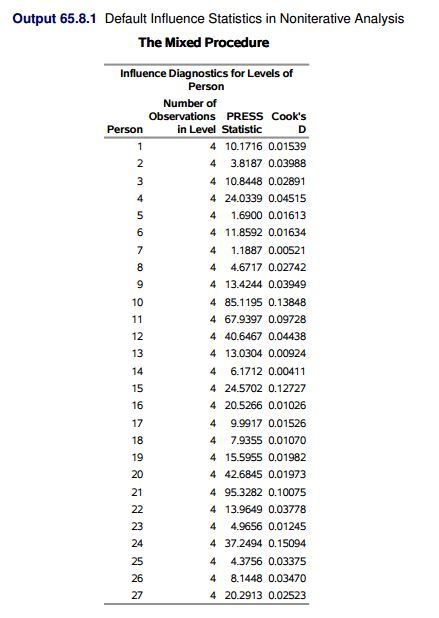
\includegraphics[width=0.7\linewidth]{images/SASoutput}
\caption{}
\label{fig:SASoutput}
\end{figure}

Each observation in the “Influence Diagnostics for Levels of Person” table in Output 65.8.1 represents the
removal of four observations. The subjects 10, 15, and 24 have the greatest impact on the fixed effects
(Cook’s D), and subject 10 and 21 have large PRESS statistics. The 21st child has a large PRESS statistic,
and its D statistic is not that extreme. This is an indication that the model fits rather poorly for this child,
whether it is part of the data or not
The previous analysis does not take into account the effect on the covariance parameters when a subject is
removed from the analysis. If you also update the covariance parameters, the impact of observations on these
can amplify or allay their effect on the fixed effects. To assess the overall influence of subjects on the analysis
and to compute separate statistics for the fixed effects and covariance parameters, an iterative analysis is
obtained by adding the INFLUENCE suboption ITER=, as follows:
\begin{verbatim}

ods graphics on;
proc mixed data=pr method=ml;
class person gender;
model y = gender age gender*age /
influence(effect=person iter=5);
repeated / type=un subject=person;
run;
\end{verbatim}
The number of additional iterations following removal of the observations for a particular subject is limited
to five. Graphical displays of influence diagnostics are created when ODS Graphics is enabled. For
general information about ODS Graphics, see Chapter 21, “Statistical Graphics Using ODS.” For specific
information about the graphics available in the MIXED procedure, see the section “ODS Graphics” on
page 5324.
The MIXED procedure produces a plot of the restricted likelihood distance (Output 65.8.2) and a panel of
diagnostics for fixed effects and covariance parameters (Output 65.8.3).
\newpage

\subsection{R Implementation}
 I am trying exercise 59.8 (page 5057) of the SAS/STAT Users Guide 12.3 in \texttt{R}. The interesting thing is that influence is investigated on subject level rather than individual level. The diagnostics in nlme does not do leave-subject-out, at least, not that I know of. MCMCglm hardly has any diagnostics. This does not mean no validation is possible, this is R, programming is not optional, but rather expected. Hence with a little bit of work it is possible to estimate PRESS, Cook's D and effects on fixed effects. From this it follows extensive validation is possible, provided we can extract the underlying variables from the model fit object.
\newpage
\subsection{Data}
Data is same as exercise 59.2 (exercise in R).
\begin{framed}
\begin{verbatim}

r1 <- read.table(textConnection('
1 F 21.0 20.0 21.5 23.0
2 F 21.0 21.5 24.0 25.5
3 F 20.5 24.0 24.5 26.0
4 F 23.5 24.5 25.0 26.5
5 F 21.5 23.0 22.5 23.5
6 F 20.0 21.0 21.0 22.5
7 F 21.5 22.5 23.0 25.0
8 F 23.0 23.0 23.5 24.0
9 F 20.0 21.0 22.0 21.5
10 F 16.5 19.0 19.0 19.5
11 F 24.5 25.0 28.0 28.0
12 M 26.0 25.0 29.0 31.0
13 M 21.5 22.5 23.0 26.5
14 M 23.0 22.5 24.0 27.5
15 M 25.5 27.5 26.5 27.0
16 M 20.0 23.5 22.5 26.0
17 M 24.5 25.5 27.0 28.5
18 M 22.0 22.0 24.5 26.5
19 M 24.0 21.5 24.5 25.5
20 M 23.0 20.5 31.0 26.0
21 M 27.5 28.0 31.0 31.5
22 M 23.0 23.0 23.5 25.0
23 M 21.5 23.5 24.0 28.0
24 M 17.0 24.5 26.0 29.5
25 M 22.5 25.5 25.5 26.0
26 M 23.0 24.5 26.0 30.0
27 M 22.0 21.5 23.5 25.0
'),col.names=c('Person','Gender','Age8','Age10','Age12','Age14'),
colClasses=c('factor','factor',rep('numeric',4)))

\end{verbatim}
\end{framed}

\begin{framed}
\begin{verbatim}

rm <- reshape(r1,direction='long',
    varying=list(c('Age8','Age10','Age12','Age14')),
    timevar='Age',idvar=c('Person','Gender'),
    v.names='y',
    times=c(8,10,12,14))
rm$Gender <- relevel(rm$Gender,ref='M')
rm$fage=factor(rm$Age)
rm$Person <- factor(rm$Person,levels=format(1:27,trim=TRUE))
rm <- rm[order(rm$Person,rm$Age),]
\end{verbatim}
\end{framed}

\begin{verbatim}
> head(rm)
Person Gender Age    y fage
1.F.8       1      F   8 21.0    8
1.F.10      1      F  10 20.0   10
1.F.12      1      F  12 21.5   12
1.F.14      1      F  14 23.0   14
2.F.8       2      F   8 21.0    8
2.F.10      2      F  10 21.5   10

\end{verbatim}


%==========================================%
Analysis, standard plot are not too difficult.

\begin{framed}
\begin{verbatim}
library(nlme)
lSymm <- lme(y ~  Age * Gender,

    data=rm, random= list(Person =pdSymm(~ fage-1)),method='ML')


plot(lSymm, resid(., type = "p") ~ Age | Person)


\end{verbatim}
\end{framed}
\begin{figure}[h!]
\centering
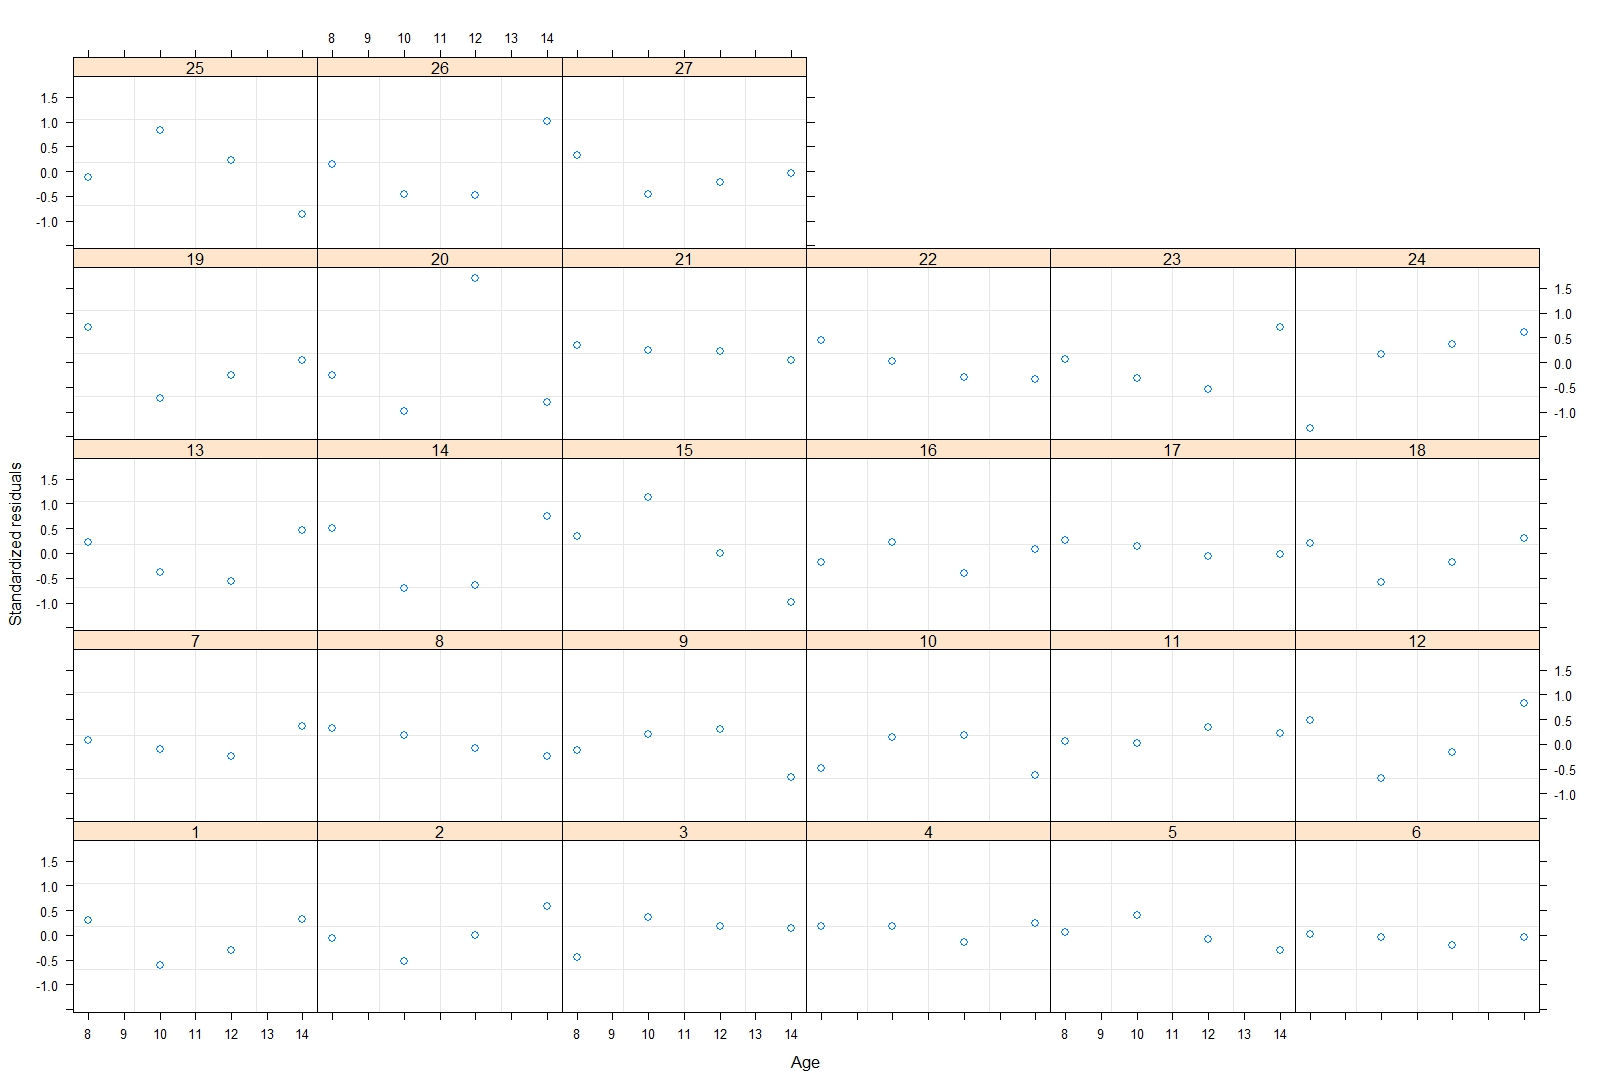
\includegraphics[width=0.99\linewidth]{images/RbloggersPlot1}
%\caption{}
%\label{fig:RbloggersPlot1}
\end{figure}
\newpage
\subsection{Subject level influence}

I have chosen to display three items, PRESS, Cook's D and effect on fixed parameters. PRESS is reasonable straightforward, the numbers more or less match. Cook's D on the other hand, is not. I took the formula of the SAS/STAT guide, which calculated it, my wording, as Mahalanobis distance of leave-subject-out fixed parameters. However, the numbers don't match. Part of that may be that I do recalculate random parameters too. Compare my figure with Output 59.8.3 top left, this seems quite similar. 

\begin{framed}
\begin{verbatim}
coefFulllme <- as.numeric(coef(lSymm)[1,1:4])

VCMlme <- vcov(lSymm)


# > VCMlme
# (Intercept)          Age     GenderF  Age:GenderF
# (Intercept)  0.87535442 -0.064802764 -0.87535442  0.064802764
# Age         -0.06480276  0.006259044  0.06480276 -0.006259044
# GenderF     -0.87535442  0.064802764  2.14859720 -0.159061330
# Age:GenderF  0.06480276 -0.006259044 -0.15906133  0.015363109


lSymmLSO <- sapply(levels(rm$Person), function(x) {

      rloo <- rm[rm$Person !=x,]

      lSymm <- lme(y ~  Age * Gender,

          data=rloo, random= list(Person =pdSymm(~ fage-1)),

          method='ML')

      coef <- as.numeric(coef(lSymm)[1,1:4])

      genderF <- rm[rm$Person==x,'Gender'][1]=='F'

      pred <- coef[1]+

          c(8,10,12,14)*coef[2]+

          genderF*coef[3]+

          c(8,10,12,14)*coef[4]*genderF

      obs <- rm[rm$Person ==x,'y']

      CD=mahalanobis(coef,coefFulllme,VCMlme)/4

      c(press=sum((obs-pred)^2),cd=CD,coef)

    })
    
\end{verbatim}
\end{framed}

\newpage

\begin{framed}
\begin{verbatim}
lSymmLSO <- t(lSymmLSO)
lSymmLSO[ ,1:2]
\end{verbatim}
\end{framed}
For the sake of brevity, here are the last ten output rows.
\begin{framed}
	\begin{verbatim}
> tail( lSymmLSO[ ,1:2] , 10)
press          cd
18  7.800734 0.007611981
19 15.196358 0.008490818
20 43.256052 0.395086129
21 96.107295 0.115497649
22 13.879678 0.033635096
23  4.961204 0.011979580
24 41.758892 0.905440147
25  4.643721 0.095851759
26  8.019698 0.026621476
27 19.920691 0.017942506

\end{verbatim}
\end{framed}

\begin{framed}
	\begin{verbatim}
plot(y=lSymmLSO[,2],x=1:27,main="Cook's D",xlab='Subject',type='h')
points(y=lSymmLSO[,2],x=1:27,main="Cook's D",xlab='Subject',type='p',pch=18,col="red")

\end{verbatim}
\end{framed}
\begin{figure}[h!]
\centering
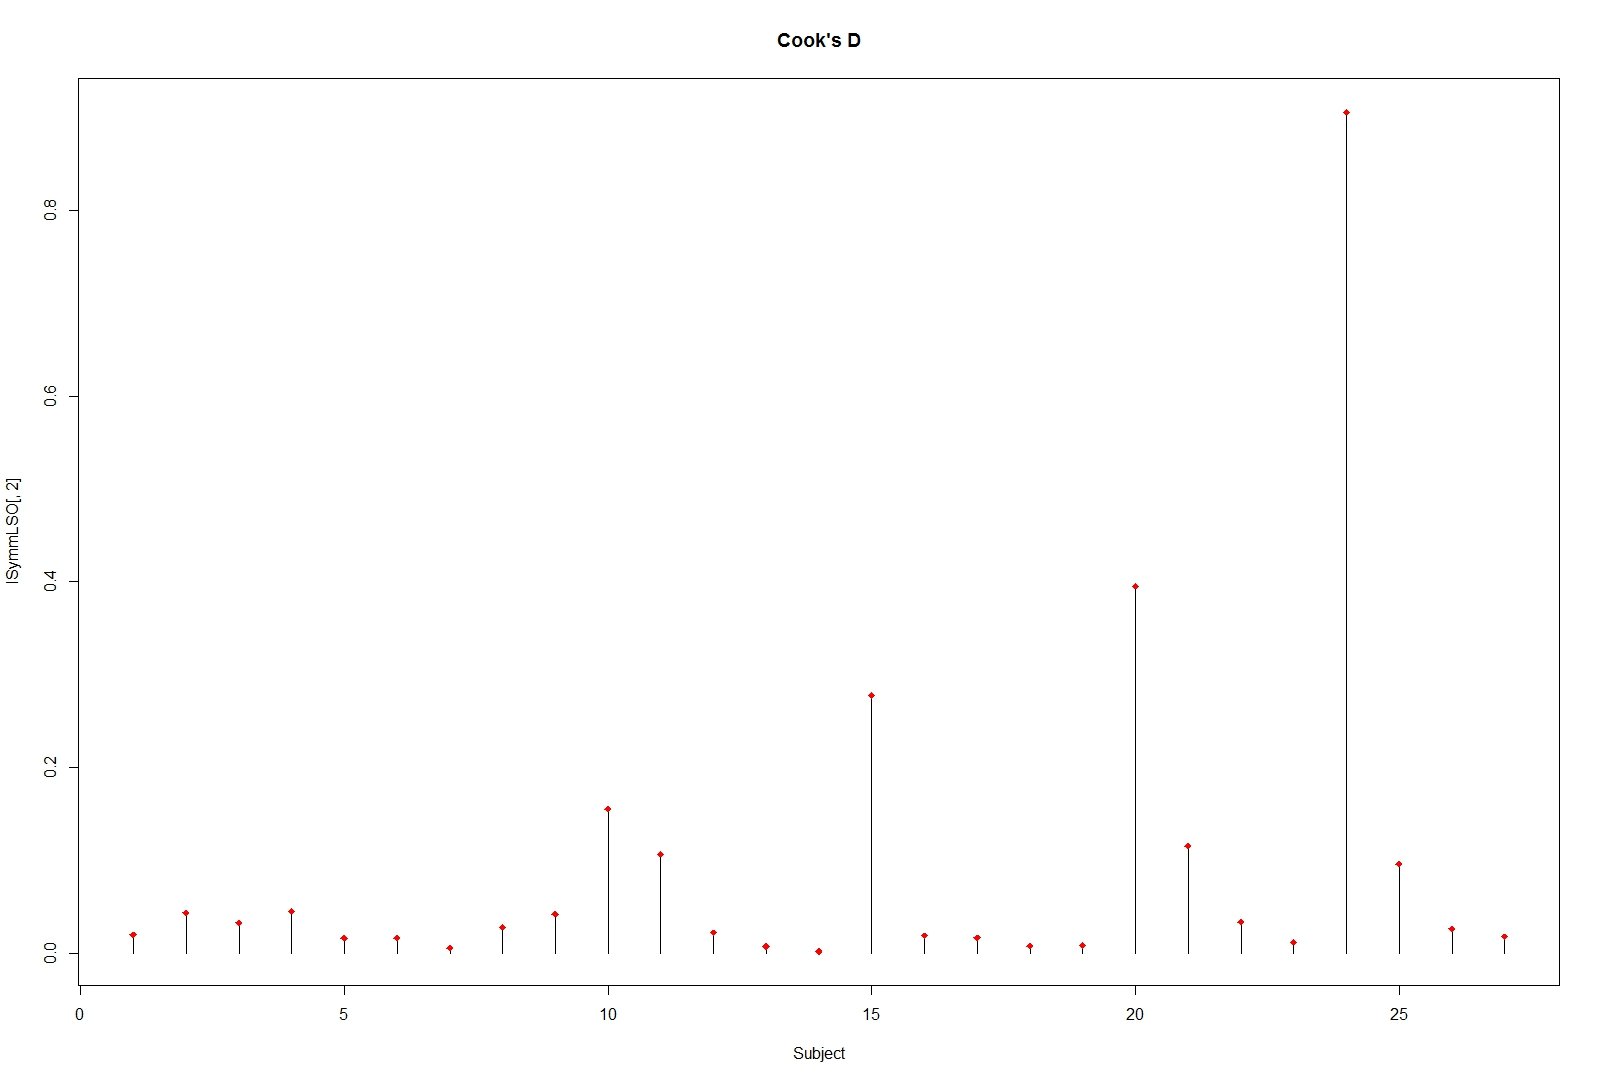
\includegraphics[width=0.7\linewidth]{images/RbloggersPlot2}

\end{figure}

\begin{figure}[h!]
	\centering
	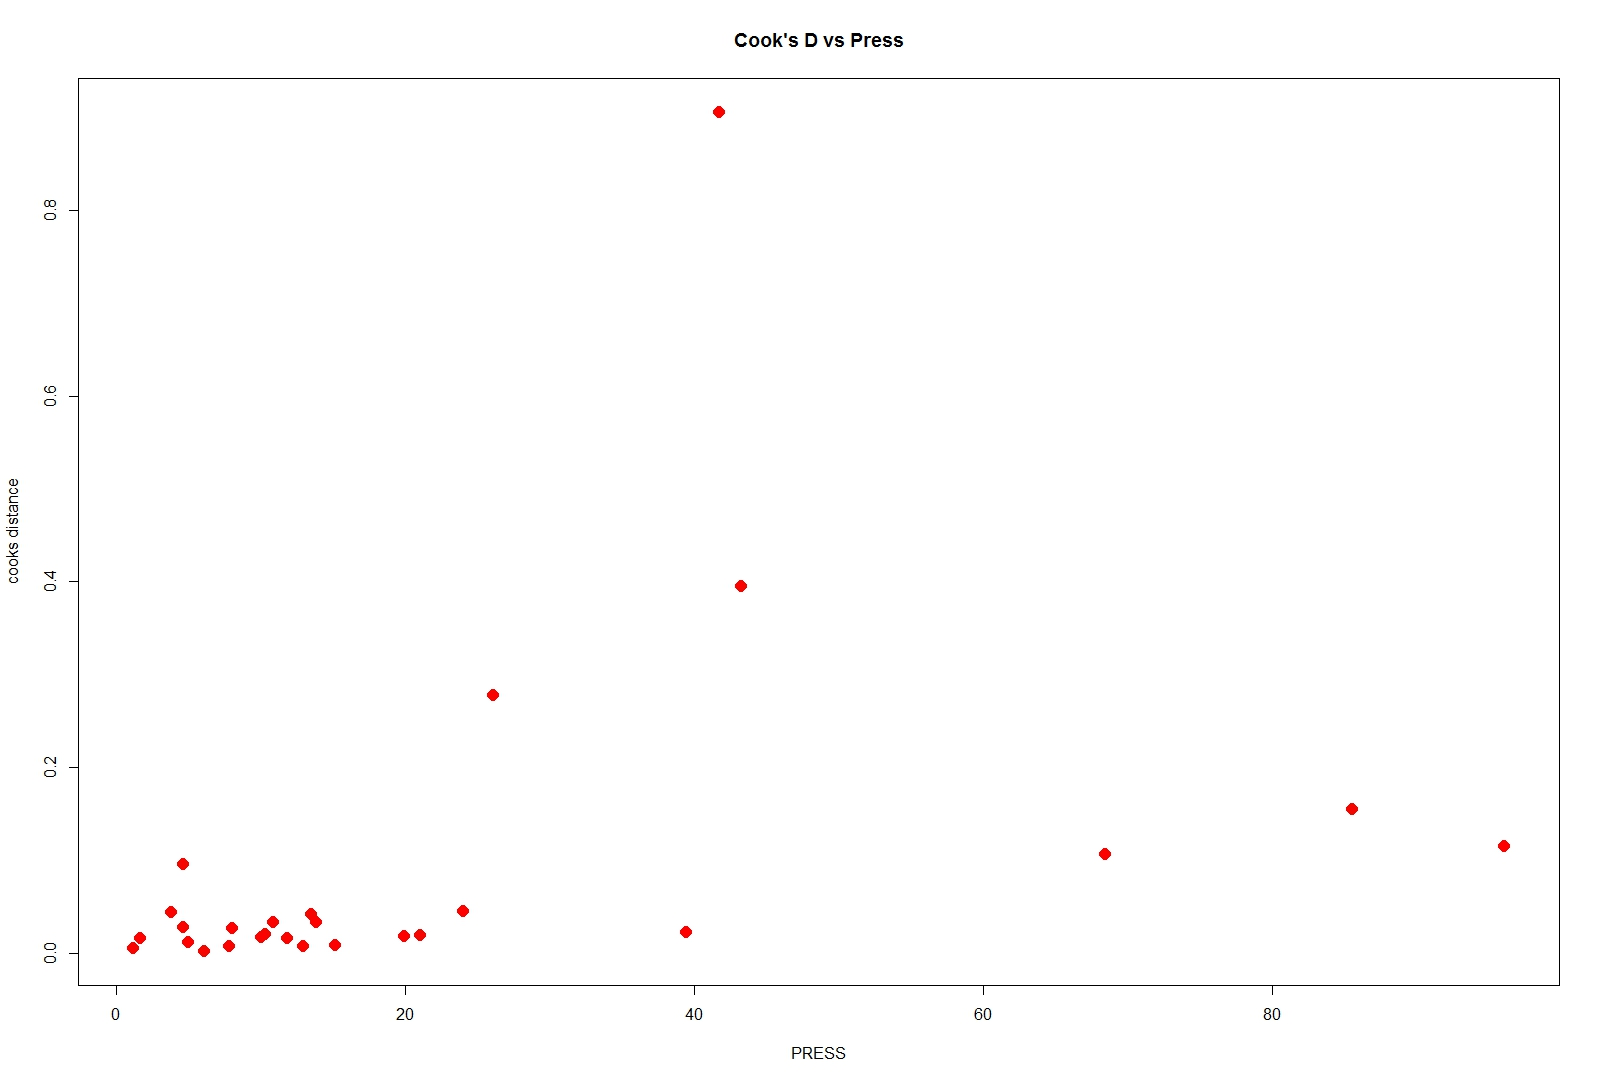
\includegraphics[width=0.7\linewidth]{images/RbloggersPlot3}
	
\end{figure}
\newpage
\subsection{Fixed-Effects Deletion Estimates}

Having done all the pre-work, the fixed effects deletion statistics are just a plot away.They do look slightly different from PROC MIXED as the model is a bit different in the SAS/STAT Guide.
\begin{framed}
	\begin{verbatim}

par(mfrow=c(2,2))

dummy <- sapply(1:4,function(x) {

  plot(y=lSymmLSO[,x+2],x=1:27,main=names(coef(lSymm))[x],ylab='',xlab='Subject')

  abline(h=coefFulllme[x])

})

\end{verbatim}
\end{framed}


\begin{figure}
\centering
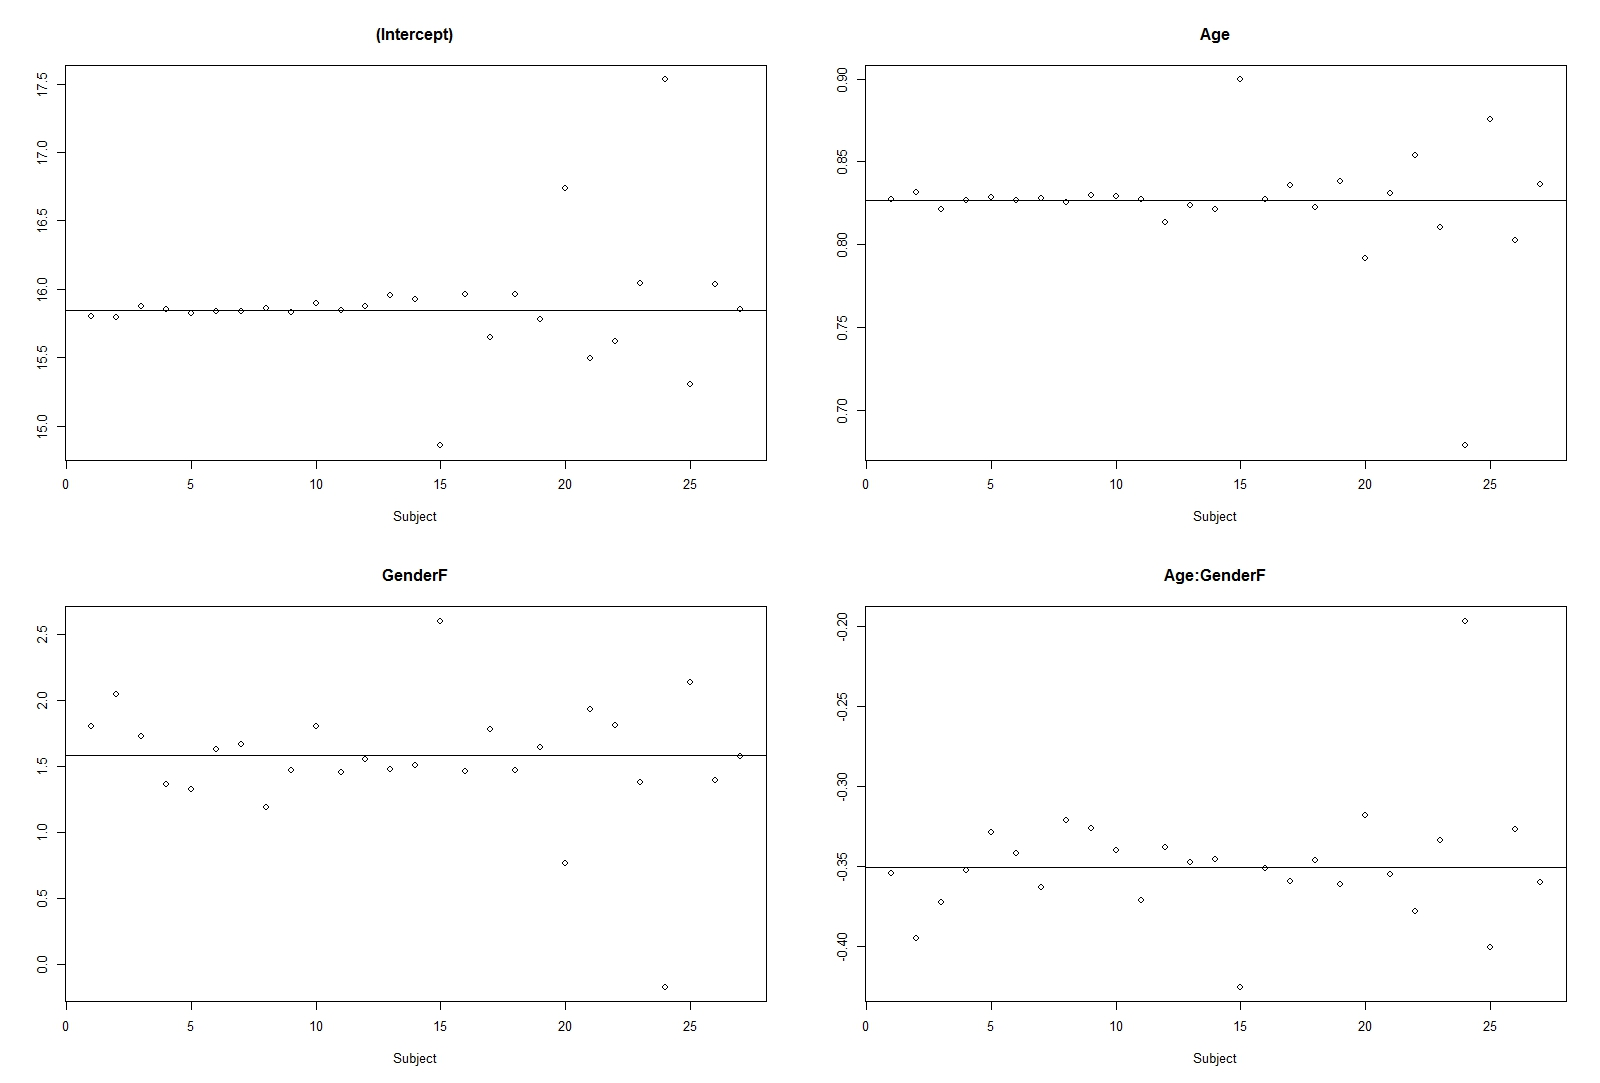
\includegraphics[width=0.7\linewidth]{images/RbloggersPlot4}
\caption{}
\label{fig:RbloggersPlot4}
\end{figure}


\subsection{MCMCglm}

The model is easy enough to fit. The approach used in nlme is easy enough to convert. Only first 5 subject's data shown for brevity. 

\begin{framed}
	\begin{verbatim}
	
library(MCMCglmm)	
	
	prior1 <- list(R=list(V=diag(4),nu=.01),
    G=list(G1=list(V=diag(1),nu=.01) ))

\end{verbatim}
\end{framed}

\begin{verbatim}
> prior1
$R
$R$V
[,1] [,2] [,3] [,4]
[1,]    1    0    0    0
[2,]    0    1    0    0
[3,]    0    0    1    0
[4,]    0    0    0    1

$R$nu
[1] 0.01


$G
$G$G1
$G$G1$V
[,1]
[1,]    1

$G$G1$nu
[1] 0.01

\end{verbatim}

\begin{framed}
	\begin{verbatim}
m1 <- MCMCglmm(y ~ Age* Gender , 
    random= ~ Person ,
    rcov=~ us(fage) :Person,
    data=rm,family='gaussian',
    nitt=500000,thin=20,burnin=50000,
    verbose=FALSE
 ,   prior=prior1
)
\end{verbatim}
\end{framed}

\begin{verbatim}

> summary(m1)

Iterations = 50001:499981
Thinning interval  = 20
Sample size  = 22500 

DIC: 122.9287 

G-structure:  ~Person

post.mean l-95% CI u-95% CI eff.samp
Person     4.222    2.034    6.874     6387

R-structure:  ~us(fage):Person

post.mean l-95% CI u-95% CI eff.samp
8:8.Person      2.6452  0.32083   5.6106    456.4
10:8.Person    -0.5309 -1.92814   0.9496    602.9
12:8.Person     0.4166 -1.48035   2.8015    434.0
14:8.Person    -0.7591 -2.32263   1.0064    594.7
8:10.Person    -0.5309 -1.92814   0.9496    602.9
10:10.Person    1.4521  0.03047   3.3624    428.2
12:10.Person   -0.4711 -1.97060   1.1899    643.0
14:10.Person    0.1578 -1.09865   1.7728    520.9
8:12.Person     0.4166 -1.48035   2.8015    434.0
10:12.Person   -0.4711 -1.97060   1.1899    643.0
12:12.Person    3.1513  0.55445   6.4259    549.2
14:12.Person    0.7605 -0.98999   3.0711    516.9
8:14.Person    -0.7591 -2.32263   1.0064    594.7
10:14.Person    0.1578 -1.09865   1.7728    520.9
12:14.Person    0.7605 -0.98999   3.0711    516.9
14:14.Person    2.0289  0.29857   4.4075    615.5

Location effects: y ~ Age * Gender 

post.mean l-95% CI u-95% CI eff.samp  pMCMC    
(Intercept)   15.8643  13.6506  18.0950    11707 <4e-05 ***
Age            0.8265   0.6481   1.0159    22500 <4e-05 ***
GenderF        1.5702  -1.7959   4.9877    21631 0.3490    
Age:GenderF   -0.3510  -0.6338  -0.0736    22500 0.0141 *  
---
Signif. codes:  0 ‘***’ 0.001 ‘**’ 0.01 ‘*’ 0.05 ‘.’ 0.1 ‘ ’ 1
> 

\end{verbatim}

\begin{framed}
	\begin{verbatim}


VCMM1 <- cov(m1$Sol)
coefFullM1 <- colMeans(m1$Sol)
\end{verbatim}
\end{framed}

\begin{verbatim}
> VCMM1 
(Intercept)          Age     GenderF  Age:GenderF
(Intercept)  1.26937339 -0.091886652 -1.28533882  0.092980766
Age         -0.09188665  0.008645708  0.09305068 -0.008769445
GenderF     -1.28533882  0.093050682  2.93663482 -0.211071425
Age:GenderF  0.09298077 -0.008769445 -0.21107143  0.019932764
> 
> coefFullM1
(Intercept)         Age     GenderF Age:GenderF 
15.8643063   0.8265224   1.5702003  -0.3509745 

\end{verbatim}

\begin{framed}
	\begin{verbatim}
m1LSO <- sapply(levels(rm$Person), function(x) {

      rloo <- rm[rm$Person !=x,]

      m1 <- MCMCglmm(y ~ Age* Gender , 

          random= ~ Person ,

          rcov=~ us(fage) :Person,

          data=rloo,family='gaussian',

     nitt=500000,thin=20,burnin=50000,

          verbose=FALSE

          ,   prior=prior1

      )

      coef <- colMeans(m1$Sol)

      genderF <- rm[rm$Person==x,'Gender'][1]=='F'

      pred <- coef[1]+

          c(8,10,12,14)*coef[2]+

          genderF*coef[3]+

          c(8,10,12,14)*coef[4]*genderF

      obs <- rm[rm$Person ==x,'y']

      CD=mahalanobis(coefFullM1,coef,VCMM1)/4

      c(press=sum((obs-pred)^2),cd=CD,coef)

    })

m1LSO <- t(m1LSO)

m1LSO[1:5,1:2]

\end{verbatim}
\end{framed}
\begin{framed}
	\begin{verbatim}
      press         cd

1 10.133019 0.01117458

2  3.835048 0.03347745

3 10.891120 0.02740768

4 24.167881 0.03618814

5  1.694508 0.01317537


\end{verbatim}
\end{framed}
For both PRESS and Cook's D it is close. For completeness the plot.Not exactly the same, but the trend and interpretations are clear enough.
\begin{framed}
	\begin{verbatim}
plot(y=m1LSO[,2]*4,x=1:27,main="Cook's D",xlab='Subject',type='h')
\end{verbatim}
\end{framed}



\begin{figure}
	\centering
	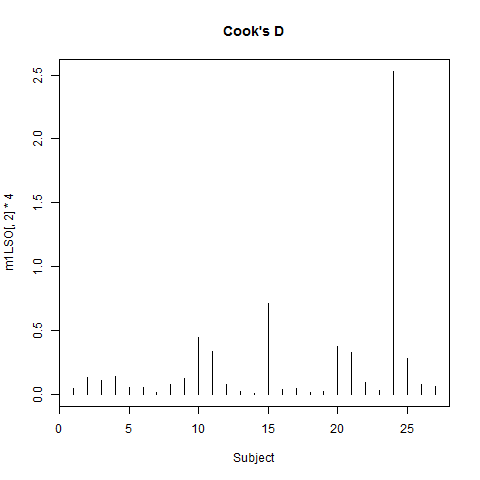
\includegraphics[width=0.7\linewidth]{images/RbloggersPNG1}
	\caption{}
	\label{fig:RbloggersPNG2}
\end{figure}




\subsection{Fixed-Effects Deletion Estimates}

Following the template from nlme, the result is similar. 

\begin{framed}
	\begin{verbatim}
par(mfrow=c(2,2))

dummy <- sapply(1:4,function(x) {

      plot(y=m1LSO[,x+2],x=1:27,main=names(coefFullM1)[x],ylab='',xlab='Subject')

      abline(h=coefFullM1[x])

    })

\end{verbatim}
\end{framed}


\begin{figure}
\centering
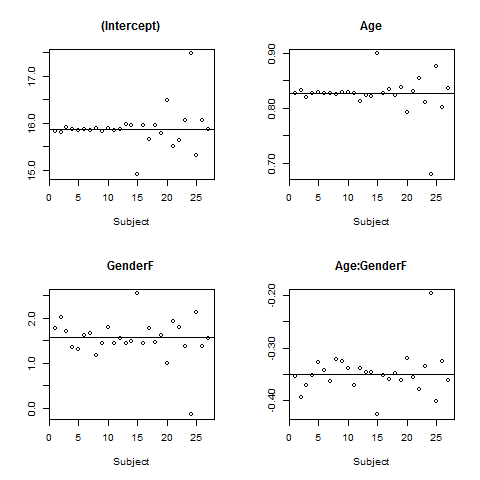
\includegraphics[width=0.7\linewidth]{images/RbloggersPNG2}
\caption{}
\label{fig:RbloggersPNG2}
\end{figure}

\end{document}